\documentclass[a4paper,10pt]{article}
\usepackage[utf8x]{inputenc}
\usepackage{cite}
\usepackage{url}
\usepackage{color}
\usepackage{graphicx}
\usepackage{hyperref}
\usepackage{fullpage}
\usepackage{enumerate}
\usepackage{amsmath}
\usepackage[italian]{babel}
\usepackage{amssymb}
\newcommand{\bra}[1]{\langle #1 |}
\newcommand{\ket}[1]{| #1 \rangle}
\newcommand{\braket}[2]{\langle #1 | #2 \rangle}
\newcommand{\ketbra}[1]{\ket{#1}\bra{#1}}

\newcommand{\sugg}[1]{\emph{Suggerimento: #1 }}
\newcommand{\mdots}[0]{\ldots\ldots\ldots\ldots\ldots\ldots\ldots\ldots\ldots\ldots\ldots\ldots}

\pdfsuppresswarningpagegroup=1

%opening

\begin{document}
%\maketitle
\section{The problem}
We consider the process
\begin{equation}
    \mu^+_1 \mu^-_2 \to \mu^+_3 \mu^-_4 X_{\ldots}\,,
    \label{eq:mumu}
\end{equation}
and we consider the limit $p_1\parallel p_3$ and $p_1\parallel p_4$.\\
We want to factorise the amplitude of proc~\ref{eq:mumu}, $A_{\mu^+\mu^-}$
in terms of $A_{\gamma\gamma}$, the amplitude of the process
\begin{equation}
    \gamma_{\tilde 1} \gamma_{\tilde 2} \to X_{\ldots}\,,
    \label{eq:aa}
\end{equation}
and suitable kernels.\\
We start from the factorisation properties of an amplitude in terms of a single collinear limit, $p_1\parallel p_3$, where
we write $A_{\mu^+\mu^-}$ in terms of  $A_{\gamma \mu^-}$. In this limt we can write
\begin{equation}
    A_{\mu^+ \mu^-} \simeq \sum_{s_1} {\overline A_{\gamma \mu^-} }_\rho\,  \epsilon(\tilde 1)^\rho_{s_1} K^{\gamma\to\mu^+\mu^-}_{s_1}\,,
    \label{eq:1split}
\end{equation}
where
\begin{itemize}
        \item $  {\overline A_{\gamma \mu^-}}_\rho$ is the amplitude for the reduced process, in this case 
            \begin{equation}
                \gamma_{\tilde 1} \mu^-_{\tilde 2} \to \mu^-_{\tilde 3} X_{\ldots}\,,
            \end{equation}
             defined as 
            \begin{equation}
             A_{\gamma \mu^-}  = {\overline A_{\gamma \mu^-}}_\rho \epsilon(\tilde 1)^\rho_{s_1}
            \end{equation}
        \item $\epsilon(\tilde 1)^\rho_{s_1}$ is the polarisation vector for a photon with momentum $p_{\tilde 1}$ and polarisation
        state $s_1 =\pm$.
        \item $ K^{\gamma\to\mu^+\mu^-}_{s_1} $ is the matrix element for the (spacelike) splitting $\gamma\to \mu^+\mu^-$.
\end{itemize}
Taking the square of Eq.~\ref{eq:1split}, we get
\begin{equation}
    A_{\mu^+ \mu^-} A_{\mu^+ \mu^-}^* \simeq 
    \sum_{s_1 t_1} {\overline A_{\gamma \mu^-} }_\rho\,  {\overline A^*_{\gamma \mu^-} }_\sigma 
    \, \epsilon(\tilde 1)^\rho_{s_1}  \epsilon^*(\tilde 1)^\sigma_{t_1} K^{\gamma\to\mu^+\mu^-}_{s_1} {K^{\gamma\to\mu^+\mu^-}}^*_{t_1}\,.
\end{equation}
The sum over polarisiations can be separated for the case where $s_1 = t_1$ and  $s_1 =- t_1$:
\begin{equation}
 \sum_{s_1 t_1} =  \sum_{s_1= t_1} + \sum_{s_1=-t_1}\,.
\end{equation}
The first term effectively sums over the polarisation of the photon, leading to a contribution
\begin{eqnarray}
   && \sum_{s_1=t_1} {\overline A_{\gamma \mu^-} }_\rho\,  {\overline A^*_{\gamma \mu^-} }_\sigma 
    \, \epsilon(\tilde 1)^\rho_{s_1}  \epsilon^*(\tilde 1)^\sigma_{t_1} K^{\gamma\to\mu^+\mu^-}_{s_1} {K^{\gamma\to\mu^+\mu^-}_{t_1}}^*\\
    &=& \sum_{s_1}{A_{\gamma \mu^-} }_{s_1}\,  {A^*_{\gamma \mu^-} }_{s_1}  K^{\gamma\to\mu^+\mu^-}_{s_1}  {K^{\gamma\to\mu^+\mu^-}_{s_1}}^*\\
    &=&\sum_{s_1}{A_{\gamma \mu^-} }_{s_1}\,  {A^*_{\gamma \mu^-} }_{s_1}  K^{\gamma\to\mu^+\mu^-}  {K^{\gamma\to\mu^+\mu^-}}^*\\
    &=& |A_{\gamma \mu^-} |^2 P^{\gamma\to\mu^+\mu^-} 
\end{eqnarray}
Where, in the second line, we have defined ${A_{\gamma \mu^-} }_{s_1} = {\overline A_{\gamma \mu^-} }_\rho\epsilon(\tilde 1)^\rho_{s_1}$;
in the third line, the independence of $|K|^2$ on $s_1$ was exploited (photon/gluon interactions conserve parity (?));
in the fourth line, we defined $|A_{\gamma \mu^-} |^2=\sum_{s_1}{A_{\gamma \mu^-} }_{s_1} {A^*_{\gamma \mu^-} }_{s_1} $
and $  P^{\gamma\to\mu^+\mu^-} =  K^{\gamma\to\mu^+\mu^-}  {K^{\gamma\to\mu^+\mu^-}}^*$.

Now, we turn to the term with different polarisations:
\begin{eqnarray}
   && \sum_{s_1=-t_1} {\overline A_{\gamma \mu^-} }_\rho\,  {\overline A^*_{\gamma \mu^-} }_\sigma 
    \, \epsilon(\tilde 1)^\rho_{s_1}  \epsilon^*(\tilde 1)^\sigma_{t_1} K^{\gamma\to\mu^+\mu^-}_{s_1} {K^{\gamma\to\mu^+\mu^-}_{t_1}}^*\\
    &=& \sum_{s_1}{A_{\gamma \mu^-} }_{s_1}\,  {A^*_{\gamma \mu^-} }_{-s_1}  K^{\gamma\to\mu^+\mu^-}_{s_1}  {K^{\gamma\to\mu^+\mu^-}_{-s_1}}^*\\
    &=&\sum_{s_1}{A_{\gamma \mu^-} }_{-s_1}\,  {A^*_{\gamma \mu^-} }_{s_1}  K^{\gamma\to\mu^+\mu^-}_{+}  {K^{\gamma\to\mu^+\mu^-}_{-}}^*\\
    &=& \tilde B^1_{\gamma \mu^-}  Q^{\gamma\to\mu^+\mu^-} 
\end{eqnarray}
W.r.t. the previous case, in the third line we assumed/exploited the independence of i
$K^{\gamma\to\mu^+\mu^-}_{\pm}  {K^{\gamma\to\mu^+\mu^-}}^*_{\mp}$ on the specific polarisation, and defined its value as
$Q^{\gamma\to\mu^+\mu^-} $ in the fourth line. Also, in the fourth line, we called 
$\tilde B^1_{\gamma \mu^-} = \sum_{s_1}{A_{\gamma \mu^-} }_{-s_1}\,  {A^*_{\gamma \mu^-} }_{s_1} $, i.e. the interference
of different polarisation states for the particle 1 in the amplitude $A_{\gamma \mu^-}$.\\
Summarising, we have obtained
\begin{equation}
  A_{\mu^+ \mu^-} \simeq  |A_{\gamma \mu^-} |^2 P^{\gamma\to\mu^+\mu^-}  +  \tilde B^1_{\gamma \mu^-}  Q^{\gamma\to\mu^+\mu^-}.
\end{equation}
The terms $P$, $Q$ are analogous to those in App.D of 0908.4272 (MadFKS) (with respect to that paper, they include the propagator of the photon). 

For the case from which we started, when both muon lines become collinear, we proceed in an analogous manner. We start from
\begin{equation}
    A_{\mu^+ \mu^-} A_{\mu^+ \mu^-}^* \simeq 
    \sum_{s_1 t_1 s_2 t_2} {\overline A_{\gamma\gamma} }_{\rho_1 \rho_2}\,  {\overline A^*_{\gamma\gamma} }_{\sigma_1\sigma_2} 
    \, \epsilon(\tilde 1)^{\rho_1}_{s_1}  \epsilon^*(\tilde 1)^{\sigma_1}_{t_1}
    \, \epsilon(\tilde 2)^{\rho_2}_{s_2}  \epsilon^*(\tilde 2)^{\sigma_2}_{t_2}
    K^{\gamma\to\mu^+\mu^-}_{s_1} {K^{\gamma\to\mu^+\mu^-}_{t_1}}^*
    K^{\gamma\to\mu^+\mu^-}_{s_2} {K^{\gamma\to\mu^+\mu^-}_{t_2}}^*\,.
\end{equation}
The sum over the four helicity indices can now be split in four terms
\begin{equation}
 \sum_{s_1 t_1 s_2 t_2} =  \sum_{s_1= t_1, s_2=t_2} + \sum_{s_1=-t_1, s_2=t_2} +\sum_{s_1= t_1, s_2=-t_2} + \sum_{s_1=-t_1, s_2=-t_2}\,.
\end{equation}
Following the same procedure as before, we obtain the following expression
\begin{equation}
  |A_{\mu^+ \mu^-} |^2 \simeq  |A_{\gamma \gamma^-} |^2 P_1 P_2  +  
                          \tilde B^1_{\gamma \mu^-}  Q_1 P_2 +
                          \tilde B^2_{\gamma \mu^-}  Q_2 P_1 +
                          \tilde B^{12}_{\gamma \gamma}  Q_1 Q_2\, .
                          \label{eq:doublecoll}
\end{equation}
We have omitted the superscript ${ }^{\gamma\to\mu^+\mu^-}$ to the $P,Q$ kernels, which now carry a subscript corresponding to the leg they refer to.

In practice, we find it practical to employ the notation of 1002.0581, in particular the configuration of our interest is Eq.~B.5 therein, which we report
here adapted to our case. In particular, for a single particle going collinear:
\begin{equation}
    |  A_{\mu^+ X} |^2= \frac{8\pi\alpha}{-k^2}\left(A_{\gamma X}A_{\gamma X}^* \right)^{\rho\sigma}\left[- g_{\rho\sigma} z + \frac{4(1-z)}{z} \hat k^\perp_\rho \hat k^\perp_\sigma\right]\,.
    \label{eq:collpwg}
\end{equation}
In this equaiton, $k^2$ is the virtuality of the photon momentum (timelike) attached to the muon line, which goes to 0 in the considered collinear limit. Using
FKS variables,  $k^2=-s \xi (1-y)/2$ .
$\left(A_{\gamma X}A_{\gamma X}^* \right)^{\rho\sigma}$ is the squared amplitude for the process where the muon line is replaced by a photon, where the photon polarization is removed; finally, $\hat k^\perp = \left(0,\cos \phi, \sin \phi,0\right)$, and $z=1-\xi$. 

If we rewrite Eq.~\ref{eq:doublecoll} in the form of Eq.~\ref{eq:collpwg}, we have, for the double-collinear limit:
\begin{eqnarray}
|A_{\mu^+ \mu^-} |^2 &=& \frac{64\pi^2\alpha^2}{k_1^2 k_2^2}
\left(A_{\gamma_1 \gamma_2}A_{\gamma_1 \gamma_2}^* \right)^{\rho_1\sigma_1\rho_2\sigma_2}
\left[g_{\rho_1\sigma_1}g_{\rho_2\sigma_2} z_1 z_2 -  
 g_{\rho_1\sigma_1} z_1 \frac{4(1-z_2)}{z_2} \hat k^{\perp2}_{\rho_2} \hat k^{\perp2}_{\sigma_2} -\right.\nonumber\\
  &&  \left.   g_{\rho_2\sigma_2} z_2 \frac{4(1-z_1)}{z_1} \hat k^{\perp1}_{\rho_1} \hat k^{\perp1}_{\sigma_1} +
\frac{4(1-z_1)}{z_1} \hat k^{\perp1}_{\rho_1} \hat k^{\perp1}_{\sigma_1}\frac{4(1-z_2)}{z_2} \hat k^{\perp2}_{\rho_2} \hat k^{\perp2}_{\sigma_2}
\right]
\end{eqnarray}
Squared amplitudes contracted with an arbirtrary vector can be obtained via MadNkLO.

\section{Numerical results}
In this section we show the collinear behaviour of the quantities to be integrated, namely matrix element ($|M|^2$), phase-space volume and Jacobian ($J$), and
their product. The title of each plot ``$A$ vs $B$'' shows the quantities compared. The color code corresponds to plotting $\log_{10} (|\frac{A}{B}-1|)$.
\begin{figure}
    \centering
    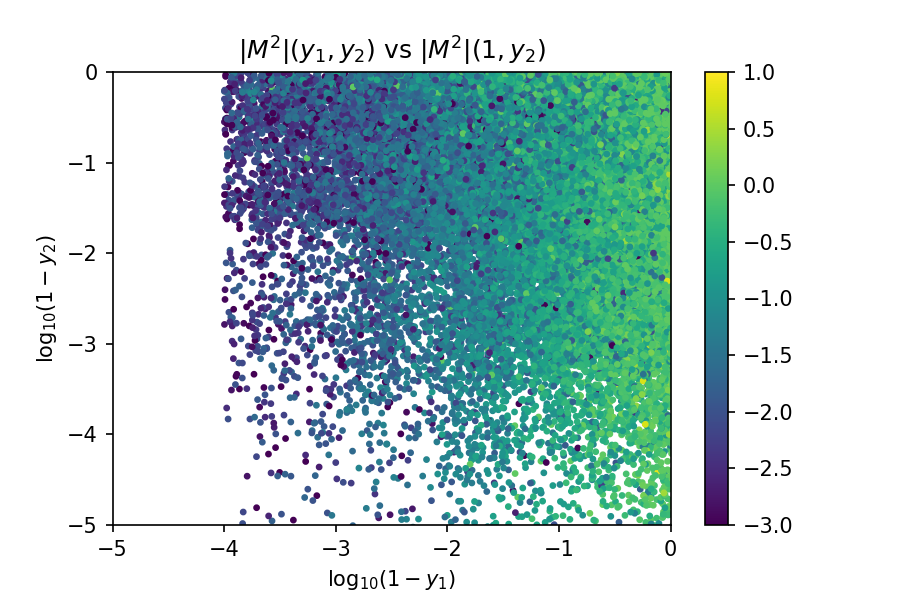
\includegraphics[width=0.4\textwidth, trim=0.2cm 0 1.8cm 0, clip]{figures/ratio_ME_0_1.png}
    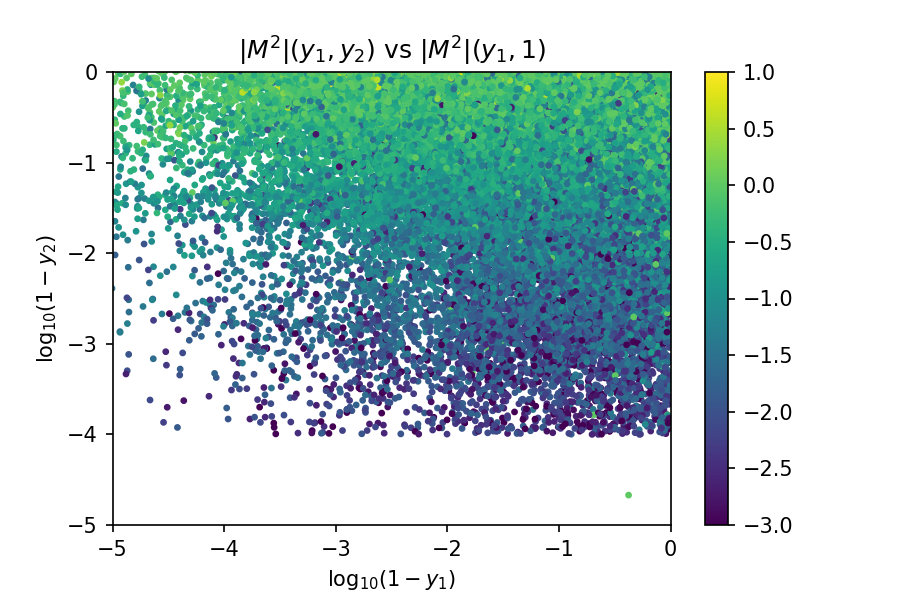
\includegraphics[width=0.4\textwidth, trim=0.2cm 0 1.8cm 0, clip]{figures/ratio_ME_0_2.png}\\
    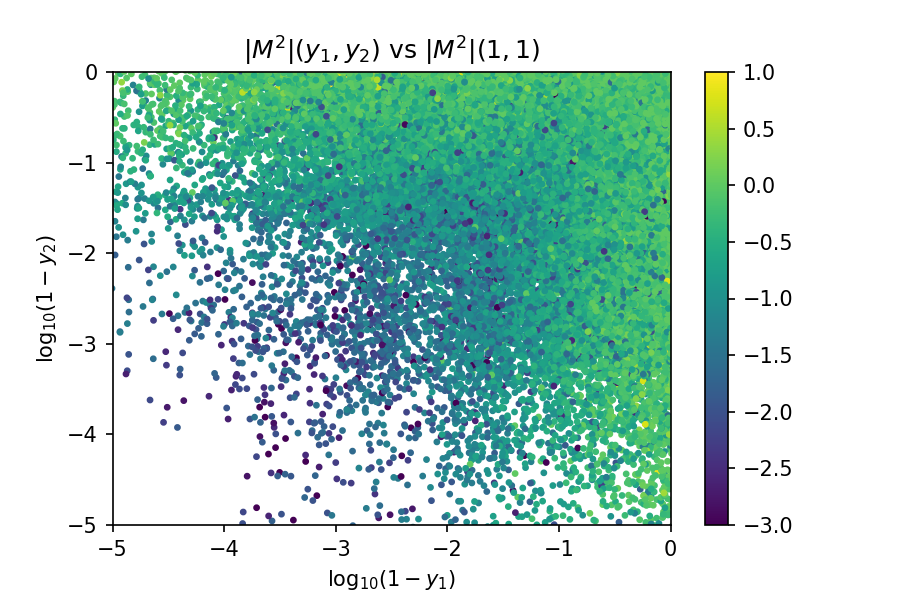
\includegraphics[width=0.4\textwidth, trim=0.2cm 0 1.8cm 0, clip]{figures/ratio_ME_0_3.png}\\
    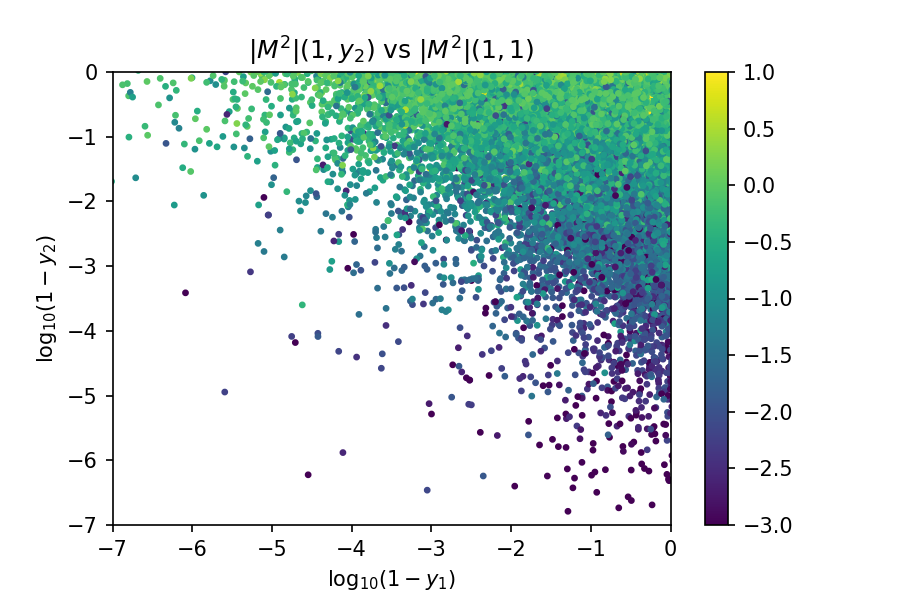
\includegraphics[width=0.4\textwidth, trim=0.2cm 0 1.8cm 0, clip]{figures/ratio_ME_1_3.png}
    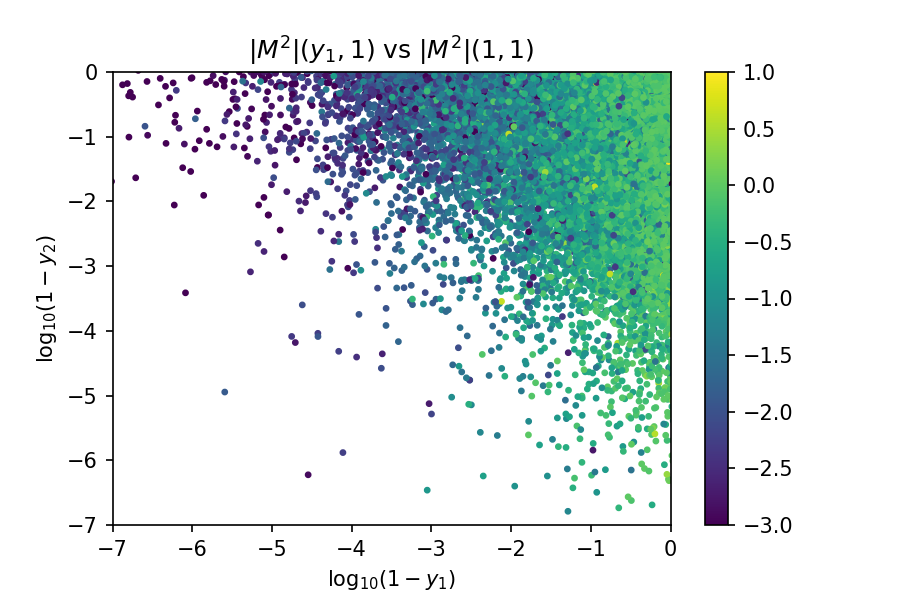
\includegraphics[width=0.4\textwidth, trim=0.2cm 0 1.8cm 0, clip]{figures/ratio_ME_2_3.png}
\end{figure}
%
\begin{figure}
    \centering
    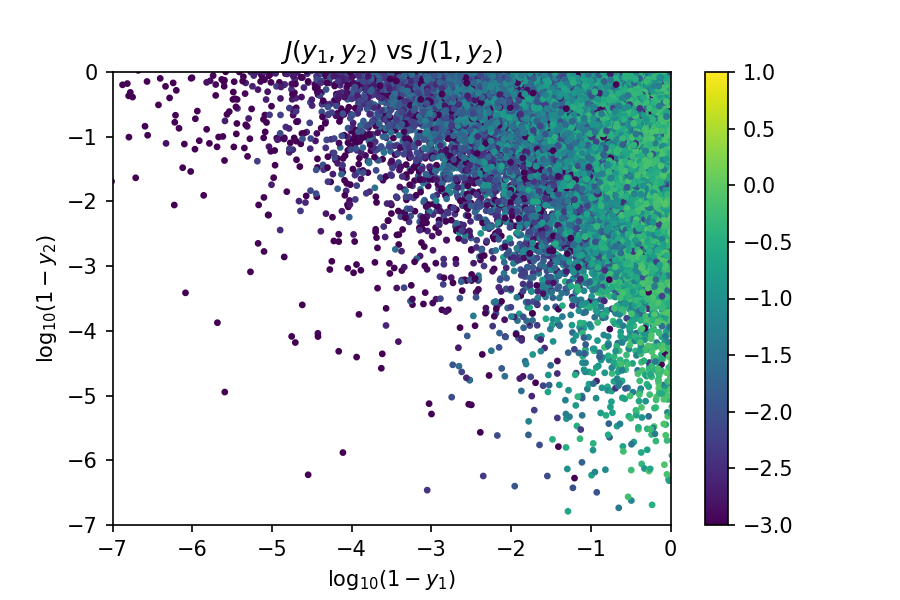
\includegraphics[width=0.4\textwidth, trim=0.2cm 0 1.8cm 0, clip]{figures/ratio_JAC_0_1.png}
    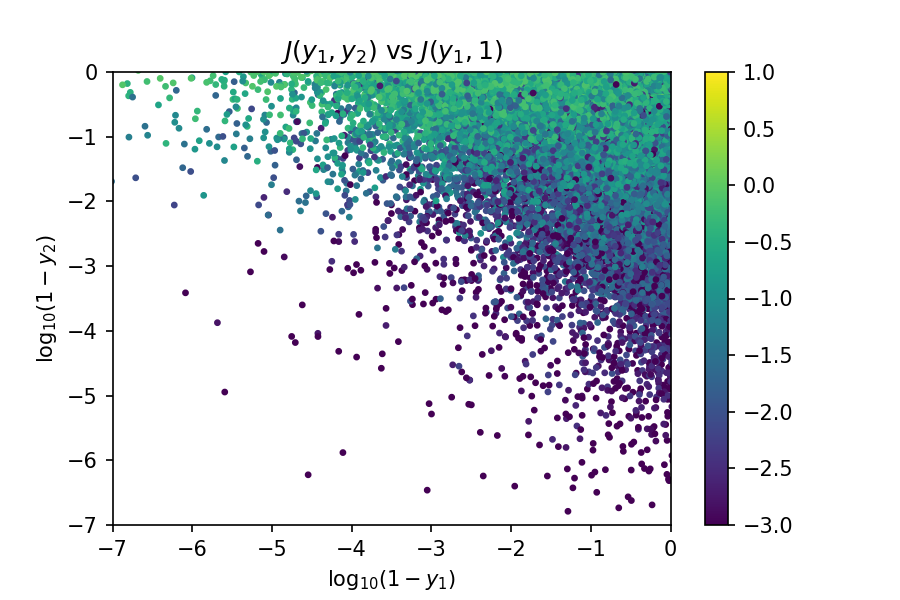
\includegraphics[width=0.4\textwidth, trim=0.2cm 0 1.8cm 0, clip]{figures/ratio_JAC_0_2.png}\\
    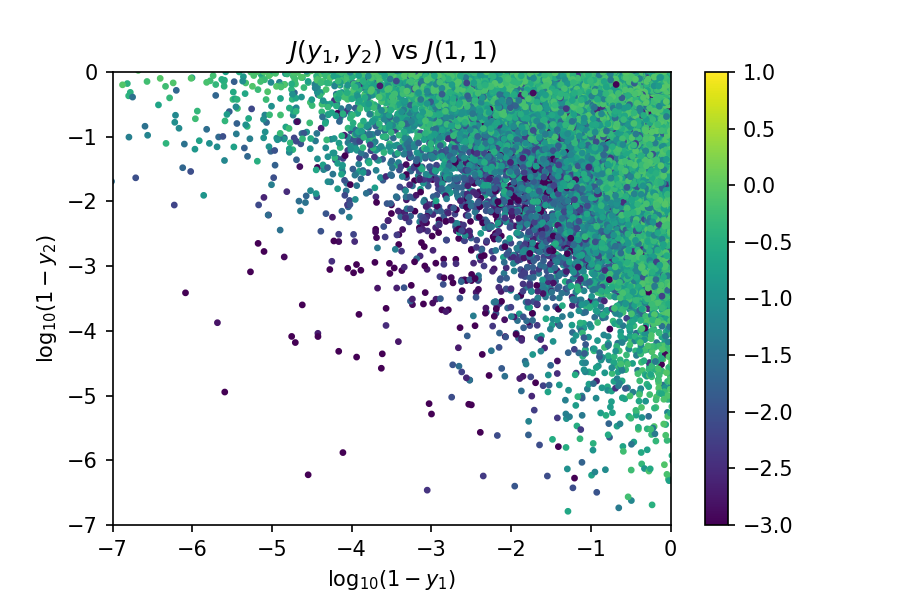
\includegraphics[width=0.4\textwidth, trim=0.2cm 0 1.8cm 0, clip]{figures/ratio_JAC_0_3.png}\\
    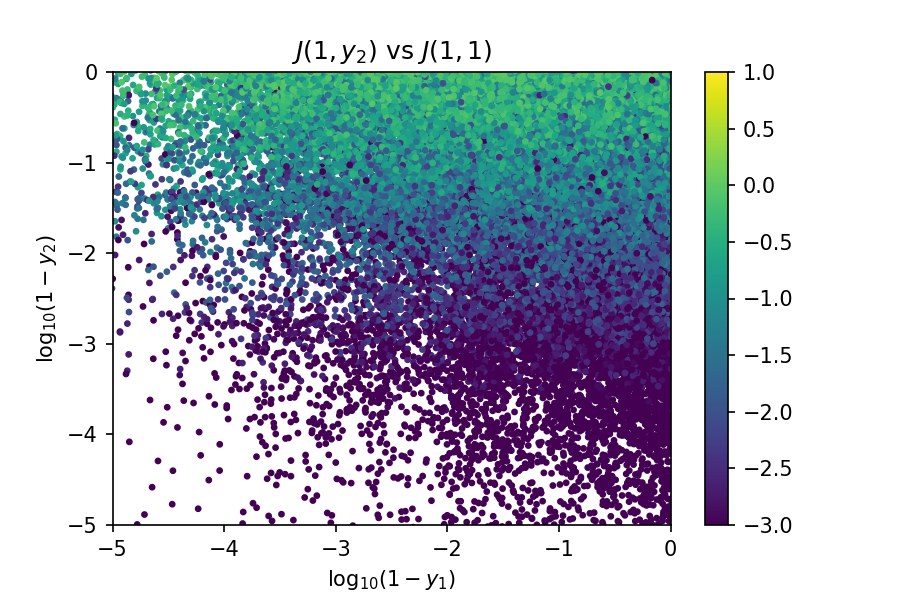
\includegraphics[width=0.4\textwidth, trim=0.2cm 0 1.8cm 0, clip]{figures/ratio_JAC_1_3.png}
    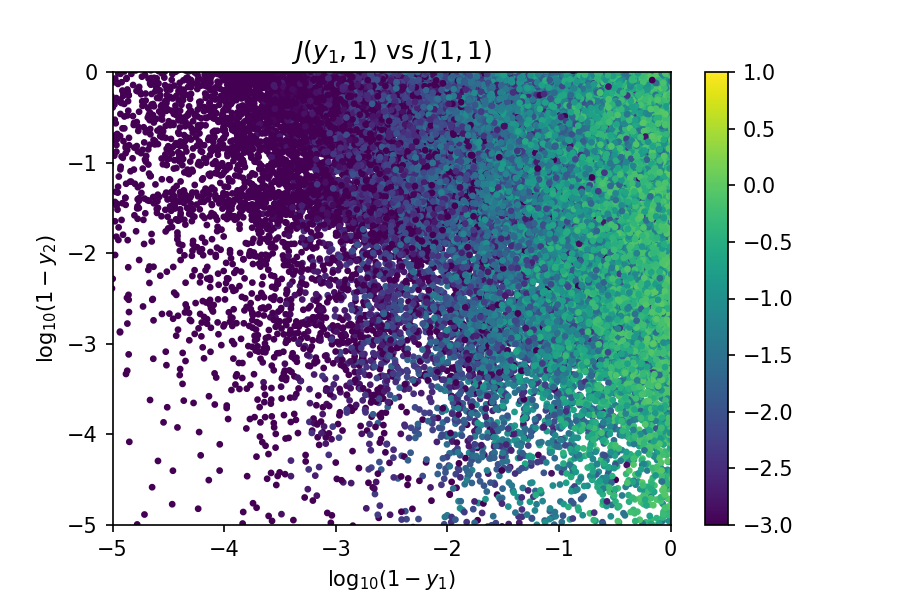
\includegraphics[width=0.4\textwidth, trim=0.2cm 0 1.8cm 0, clip]{figures/ratio_JAC_2_3.png}
\end{figure}
%
\begin{figure}
    \centering
    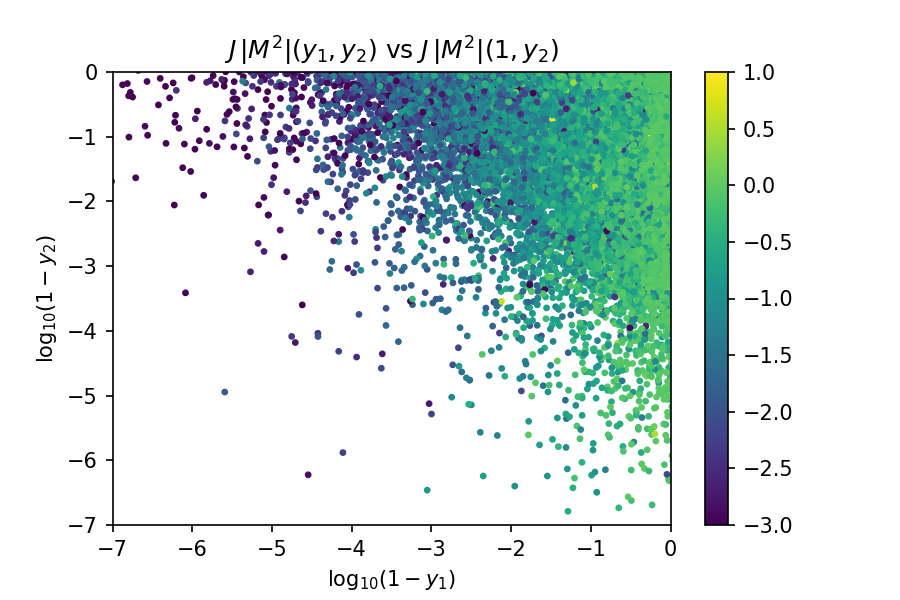
\includegraphics[width=0.4\textwidth, trim=0.2cm 0 1.8cm 0, clip]{figures/ratio_JAC.ME_0_1.png}
    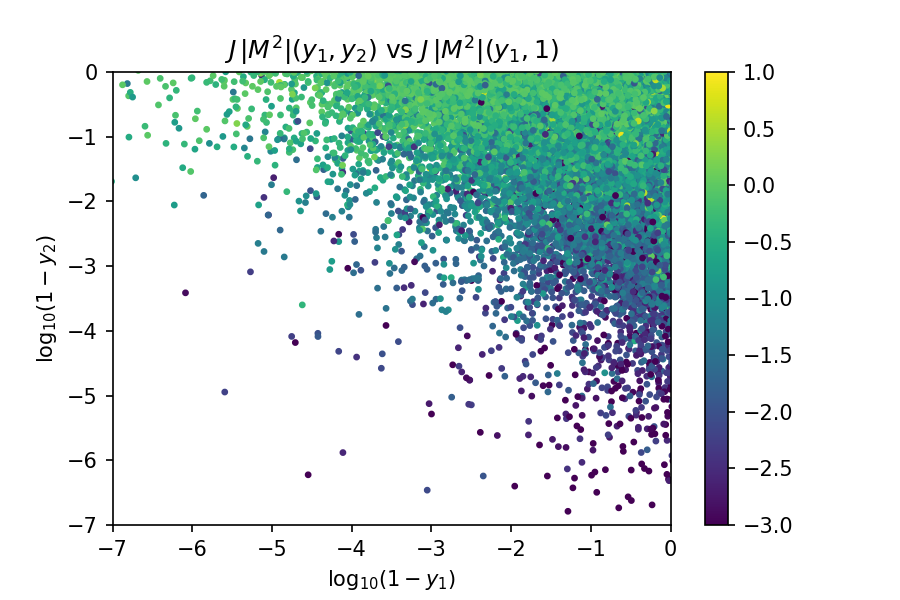
\includegraphics[width=0.4\textwidth, trim=0.2cm 0 1.8cm 0, clip]{figures/ratio_JAC.ME_0_2.png}\\
    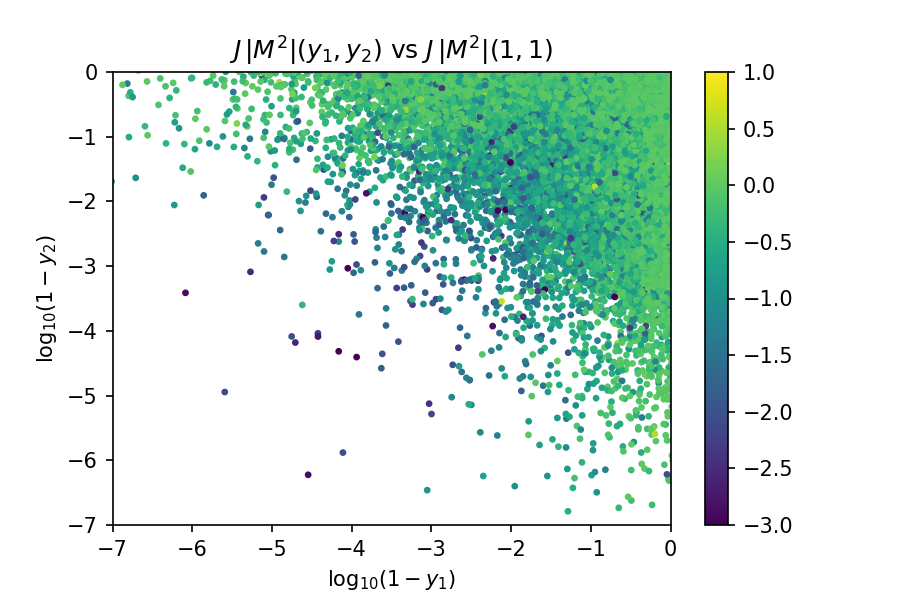
\includegraphics[width=0.4\textwidth, trim=0.2cm 0 1.8cm 0, clip]{figures/ratio_JAC.ME_0_3.png}\\
    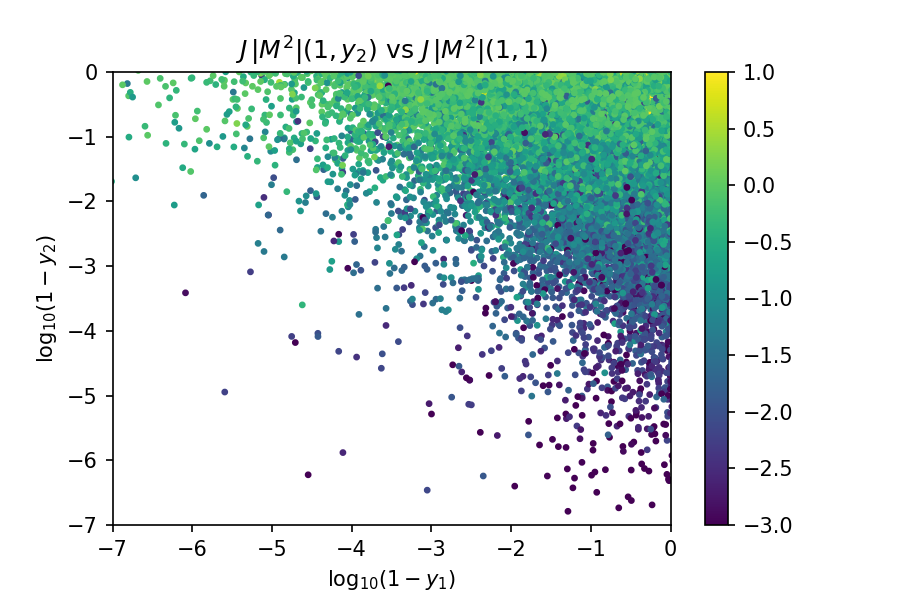
\includegraphics[width=0.4\textwidth, trim=0.2cm 0 1.8cm 0, clip]{figures/ratio_JAC.ME_1_3.png}
    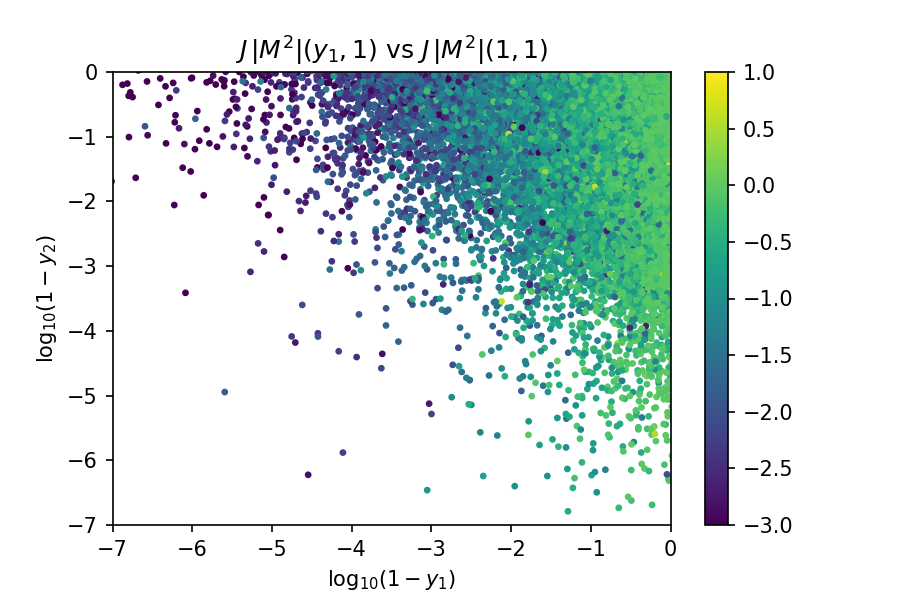
\includegraphics[width=0.4\textwidth, trim=0.2cm 0 1.8cm 0, clip]{figures/ratio_JAC.ME_2_3.png}
\end{figure}


\end{document}
